\documentclass{subfiles}

\begin{document}
    \marginnote{\textbf{\textit{VL 16}}\\22.06.2023, 10:00}
    

    \subsection{Lebensdauer angeregter Zustände und Linienbreiten}
        Unter der Lebensdauer angeregter Zustände verstehen wir die mittlere Zeit, die ein Atom im angeregten Zustand verbringt, bevor es in den Grundzustand zurückkehrt. Die spontane Emission der Photonen erfolgt durch die Wechselwirkung mit dem Vakuumfeld, dem sogenannten \emph{Vakuumfluktationsfeld}. Die Wahrscheinlichkeit eines solchen Überganges wird mit dem \textsc{Einstein-Koeffizienten} $(n,m)\mapsto A_{n\to m}$ beschrieben. Ein solcher Vorgang führt dann zur Aussendung eines Photons der Energie $(n,m)\mapsto h\cdot\nu_{n\to m}$. Es ist dann die Anzahl der Übergänge pro Zeit gegeben durch 
        \[
            \dv{t}N_n = -A_{n\to m}N_n\Longleftrightarrow \dv{t}N_n = -N_n\cdot A_n, \quad A_n:=\sum_{m\neq n}A_{n\to m}.
        \]
        Durch die Annahme von \emph{Homogenität} und \emph{Isotropie} des Vakuumfluktationsfeldes sehen wir stets diesen linearen Zusammenhang. 
        \begin{Aufgabe}
            \nr{} Recherchiere in diesem Zusammenhang die \emph{virtuellen Photonen} und den \href{https://de.wikipedia.org/wiki/Casimir-Effekt}{\emph{Casimir-Effekt}}.
        \end{Aufgabe}
        Aus der angegebenen Differentialgleichung stellt die Lösung
        \[
            N(t) = N_i(0)\cdot \exp(-A_n\cdot t),\quad N(0) = N_i(0)
        \]
        die \emph{Besetzungsfunktion} und in der Auswertung die \emph{Besetzungszahl} dar. Die mittlere Lebensdauer $\tau_n$ ist dann gegeben durch $\tau = \bbra{1/A_n}_{n\in\N}$. Führt man den Begriff der \emph{Übergangswahrscheinlichkeit} für einen weiteren Prozess ein, so ergibt sich $\dv{t}N_n = -(A_n + R_n)\cdot N_n$ und für die \emph{effektive Lebensdauer} $\tau^\textit{eff} = \bbra{1/(A_n + R_n)}_{n\in\N}$. 

        \subsubsection*{Linienbreite}
            Mittels der Heisenbergschen Unschärferelation $\Delta E\cdot\Delta t\geq\hbar/2$ hat die \emph{spektrale Linienbreite} die Form einer Gaußverteilung. Die \emph{natürliche Linienbreite} ist dabei gegeben durch $\Delta\nu = \hbar/(2\pi\tau_n)$. Hierfür muss die klassische Oszillatorgleichung $x'' + \gamma\cdot x' + \omega_0^2 x = 0$ gelöst werden:
            \[
                x(t) = x_0\cdot\exp(-\gamma t/2)\cdot\nbra{\cos(\omega t) + \frac{\gamma}{2\omega}\sin(\omega t)},\quad \omega = \sqrt{\omega_0^2 - \frac{\gamma^2}{4}}.
            \]
            Für $\gamma\ll\omega_0$ ergibt sich $\omega \approx\omega_0$ und $\gamma/(2\omega)\ll 1$, sodaß $x(t) \approx x_0\cdot\exp(-\gamma t/2)\cdot\cos(\omega t)$. Um an das Spektrum $A(\omega)$ zu gelangen, muss eine Fouriertransformation durchgeführt werden. Wir erhalten
            \[
                A(\omega) = \frac{1}{2\pi}\cdot\int_R x(t)\cdot\exp(-\cmath\omega t)\;dt,
            \]
            sodaß sich durch Einsetzen schließlich die Funktion
            \[
                A(\omega) = \frac{x_0}{\sqrt{2\pi}}\cdot\nbra{\frac{1}{\cmath\cdot(\omega_0 - \omega) + \gamma/2} + \frac{1}{\cmath\cdot(\omega_0 + \omega) + \gamma/2}}.
            \]
            In einer Umgebung von $\omega_0$ gilt damit für die Leistung $P(\omega) \propto A(\omega)\cdot (A(\omega))^*$. 

            \begin{Aufgabe}
                \nr{} Fülle die Lücken dieser Herleitung auf und bestimme $P$. Das Vorlesungsergebnis lautet dabei $P(\omega) = P_0\cdot (\gamma/(\pi2))/((\omega-\omega_0)^2 + (\gamma/2)^2)$, benannt als \href{https://de.wikipedia.org/wiki/Lorentzkurve}{\emph{Lorentz-Kurve}}. Bestimme die Halbwertsbreite $\Delta\omega = \gamma$.
                
                \nr{} Zeige an dieser Stelle den Zusammenhang zur charakteristischen Zeit $\tau = 1/\gamma$, $\tau_n = 1/A_n$ aus füheren Überlegungen. 
            \end{Aufgabe}

        \subsubsection*{Doppler Verbreiterung}
            Die \emph{Doppler Verbreiterung} ist ein Effekt, der durch die thermische Bewegung der Atome hervorgerufen wird. Die Geschwindigkeitsverteilung der Atome ist dabei durch die \emph{Maxwell-Boltzmann-Verteilung} gegeben. Für eine Atomgeschwindigkeit $v\in\R^3$ ergibt sich zunächst der \emph{Dopplereffekt} mit $\omega = \omega_0 + \scpr{k}{v}$. In die $z$ Richtung ergibt sich dann eine Verteilung 
            \[
                P(v_z) = \frac{1}{\sqrt{2\pi}\cdot\Delta v_z}\cdot\exp(-v_z^2/(2\Delta v_z^2)),\quad \Delta v_z = \sqrt{\frac{k_B\cdot T}{m}}.
            \]
            \begin{Aufgabe}
                \nr{} Führe eine Transformation auf die Frequenz durch und bestimme die Verteilung $P(\omega)$. 
            \end{Aufgabe}

    \section{Der Spin}
        \subsection{Stern-Gerlach-Experiment}
            Das \href{https://de.wikipedia.org/wiki/Stern-Gerlach-Versuch}{\emph{Stern-Gerlach Experiment}} weist die Richtungsquantelung des Drehimpulses nach. Dabei wird ein Strahl von Silberatomen durch ein inhomogenes Magnetfeld geschickt. Der schematische Aufbau des Experiments ist wiefolgt:
            \begin{figure}[]
                \centering
                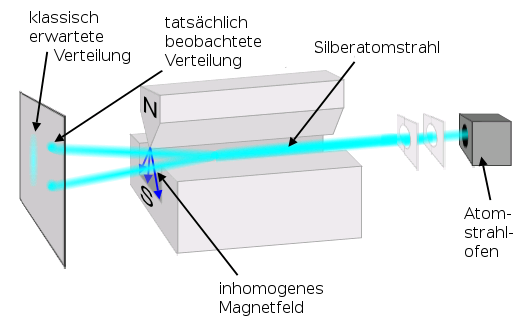
\includegraphics[width=7cm]{Bilddateien/SternGerlach.png}
                \caption{Schematischer Aufbau des Stern-Gerlach-Experiments.}
            \end{figure}
            Der Spinnachweis gelingt dabei dadurch, daß die Atome in zwei verschiedene Richtungen abgelenkt werden. 
            \begin{Aufgabe}
                \nr{} Zur Anschauung des Prizips betrachte das hinterlegte $\to$\href{https://en.wikipedia.org/wiki/File:Quantum_spin_and_the_Stern-Gerlach_experiment.ogv}{Video}.

                \nr{} Betrachte die hinterlegte $\to$\href{https://upload.wikimedia.org/wikipedia/commons/c/cb/Stern-Gerlach_Analyzer_Sequential_Series_E3.png}{Grafik} und erkläre die dazu führenden Prozesse. 
            \end{Aufgabe}



\end{document}